\documentclass[10pt,twocolumn,letterpaper]{article}

\usepackage{cvpr}
\usepackage{times}
\usepackage{epsfig}
\usepackage{graphicx}
\usepackage{amsmath}
\usepackage{amssymb}

% Include other packages here, before hyperref.

% If you comment hyperref and then uncomment it, you should delete
% egpaper.aux before re-running latex.  (Or just hit 'q' on the first latex
% run, let it finish, and you should be clear).
\usepackage[pagebackref=true,breaklinks=true,letterpaper=true,colorlinks,bookmarks=false]{hyperref}

\cvprfinalcopy % *** Uncomment this line for the final submission

\def\cvprPaperID{****} % *** Enter the CVPR Paper ID here
\def\httilde{\mbox{\tt\raisebox{-.5ex}{\symbol{126}}}}

% Pages are numbered in submission mode, and unnumbered in camera-ready
\ifcvprfinal\pagestyle{empty}\fi
\begin{document}

%%%%%%%%% TITLE
\title{
Lightweight Sentiment Analysis: Comparing Small LLMs, Large Models, and Traditional ML Approaches

Small NLP: CS 7643
}

\author{
Jaden Zwicker, 
Houshmand Abbaszadeh,
Third Author 
\\
Georgia Institute of Technology\\
Atlanta, GA 30332\\
{\tt\small 
jzwicker3@gatech.edu, 
habbaszadeh6@gatech.edu, 
thirdauthoremail@gatech.edu}
% For a paper whose authors are all at the same institution,
% omit the following lines up until the closing ``}''.
% Additional authors and addresses can be added with ``\and'',
% just like the second author.
% To save space, use either the email address or home page, not both
}



\maketitle
%\thispagestyle{empty}

%%%%%%%%% ABSTRACT
\begin{abstract}
Recent advancements in large language models (LLMs) have set unprecedented benchmarks in sentiment analysis, but their exceptional performance often comes at the cost of significant computational resources. This project investigates the viability of a lightweight, fine-tuned deep learning model capable of running on modest hardware, as a cost-effective alternative to models like BERT and GPT. Using IMDb’s movie review dataset \cite{IMDB-dataset}, we evaluate the performance of a 135M-parameter small LLM, “SmolLM,” leveraging few-shot learning and fine-tuning to improve its sentiment analysis capabilities.

The project benchmarks SmolLM against state-of-the-art LLMs, non-transformer deep learning networks such as CNNs and LSTMs, and traditional machine learning approaches like Logistic Regression, Naive Bayes, and Random Forests. Performance metrics are derived from internal experimentation as well as from existing literature on this well-studied dataset.

Our goal is to demonstrate how fine-tuned small models can offer a competitive alternative to traditional methods and larger LLMs for relatively simple NLP tasks. In addition, we explore the diminishing returns of computationally intensive models, highlighting the potential to reduce deployment and operational costs without sacrificing performance. The outcomes of this work aim to guide practitioners in balancing accuracy with resource efficiency in sentiment analysis tasks.

\end{abstract}

%%%%%%%%% BODY TEXT
\section{Introduction/Background/Motivation}
\textbf{MENTION THE PARAM SIZE OF THE MODELS AND TIE IT BACK TO THE PROBLEM WE ARE SOLVING AND WHAT DIFF IT WILL MAKE}

This project aims to compare the performance and computational costs of small and large language models for sentiment analysis on the IMDb movie reviews dataset \cite{IMDB-dataset}. The objective is to demonstrate that simpler models, when properly tuned, can deliver competitive performance without the need for expensive computational resources. This project will also explore how the small and large language models compare to traditional machine learning models like naive bayes, logistic regression, and random forest learners. By showcasing the effectiveness of lightweight models, we seek to address the widespread over-reliance on large, resource-intensive models and provide a sufficient and cost effective alternative. 

Furthermore the source of the small models, which we sought to fine tune, mentions that they were specifically designed for this type of use case \cite{hf-smollm-usecase}. In their analysis they mention that iPhone 15 Pros have 8GB of DRAM which is sufficient to run all three of their SmolLM2 Models \cite{hf-smollm2-collection}. With this they provide a memory footprint, which is in Figure \ref{fig:smollm-memory}, of the models in their default configurations proving just how little computational resources are needed to run these models which we hope to get to a point of comparable performance to larger industry grade LLMs.

In today's world, sentiment analysis for simple tasks like review
classification is often performed using heavy-weight models such as BERT and GPT. The limits of the current practice include longer training and inference times, higher energy consumption, and restricted accessibility for smaller organizations or individuals. These models also require expensive hardware and consume significant computing resources, making them costly to implement. This approach is extremely resource intensive for straightforward tasks,
whereas lightweight models can achieve competitive results at a fraction of the cost and training time.


\subsection{Why this project matters}
If this project succeeds, and the SmolLM is able to achieve competitive results, then this will provide a means for small businesses and even individuals to implement simple sentiment analysis without the need for advanced hardware or significant computing resources. Sentiment analysis would become more accessible and usable to a wider range of clients, improving their business insights and application capabilities

\begin{figure}[t]
\begin{center}
% \fbox{\rule{0pt}{2in} \rule{0.9\linewidth}{0pt}}
\fbox{
    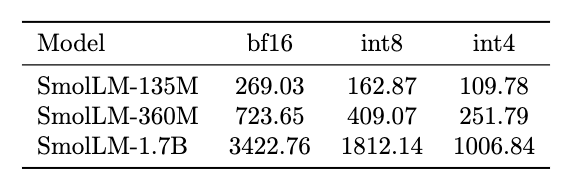
\includegraphics[width=0.8\linewidth]{figures/smollm-memory.png}
}
\end{center}
   \caption{Memory footprint of SmolLM models \cite{hf-smollm-usecase}.}
\label{fig:smollm-memory}
\end{figure}


\begin{figure}[t]
\begin{center}
% \fbox{\rule{0pt}{2in} \rule{0.9\linewidth}{0pt}}
\fbox{
    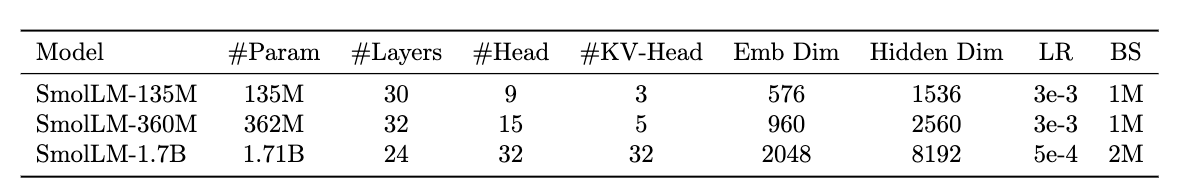
\includegraphics[width=1\linewidth]{figures/smollm-params.png}
}
\end{center}
   \caption{Architecture details of SmolLM models \cite{hf-smollm-usecase}.}
\label{fig:smollm-parameteres}
\end{figure}


\subsection{Dataset Selection}
The dataset chosen to test the various models sentiment analysis capabilities was the IMDb's movie Review dataset \cite{IMDB-dataset}. This dataset contains strings of movie reviews, which was pulled from IMDb's website in 2011 making it a sample of the total amount of reviews they store. Each movie review sample is accompanied by the dataset's binary sentiment classification of Positive or Negative. The dataset contains 50,000 total samples with 25,000 being for training and 25,000 for testing with an approximately 50/50 split between Positive and Negative classifications. These specifics of the dataset make it very balanced leading to it being well tested in literature and the perfect benchmark for basic sentiment analysis. Given the datasets format as strings already and it being from the same creators as the models we were testing no pre-processing was needed outside of tokenizing each input prompt before feeding it into the language models. 




%------------------------------------------------------------------------
\section{Approach}

\textbf{Mention the models were run on A100 with 40gb for consistency among tests}


\subsection{SmolLM Choice}
Talk about why we chose the models in more detail for fine tuning and beating LLMs, ie small and can run on phone and open source. Cite this \cite{hf-smollm-usecase}.
Also, mention why 135M over the other models

\textbf{Important: Mention any code repositories (with citations) or other sources that you used, and specifically what changes you made to them for your project. }



\subsection{Generating SmolLM Benchmarks}
To first investigate or compare the variety of models mentioned some initial tests and benchmarking had to be done. While traditional ML techniques for sentiment analysis and well documented LLMs have existing literature providing metrics for them running on the IMDb dataset \cite{IMDB-dataset} our choice for tuning a SmolLM model would require us to determine the baseline performance. Hence one of the first goals of this project was to test all three sizes of SmolLM models in both zero-shot and few-shot scenarios so later comparisons could better be made. This benchmarking was done on the 25,000 test samples from the dataset with each sample getting its own individual prompt to the model (no batching was used). 

An initial problem which was quickly realized from the zero-shot testing was that the SmolLM models did not always return a clear Positive or Negative classification of the movie prompt. Since no previous examples of answering the question were given (few-shot did this) the smaller sized models such as SmolLM-135M would simple repeat the question back or answer with random commonly used words such as 'I' or The repeatedly. To accommodate for this issue our initial approach had to be adjusted. Rather then parse the full reply that the models generated we took the top 50 most probable next words (logits) that the model generated and parsed through them to see if Positive of Negative appeared and if it did the first one was taken as the models answer. This methodology keeps the premise of sentiment analysis while taking into account that LLMs can give wordy responses making it hard to determine what sentiment they actually gave the prompt. Also, if the model was unable in those 50 most likely words to give an answer of either Positive of Negative this was treated as a default Negative answer however, we tracked these scenarios to bring up in later data points and analysis. 

Another initial testing issue that arouse, all of which allowed us to learn about the models better before fine tuning, was the dependence on the prompting method for determining the Models response. For example, if the prompt was phrased as follows: \textit{\textbf{"Only Answer if this Movie Review is Positive or Negative:"}} then the smaller models would be more likely to select the first mentioned classification. So if the prompt asked Positive vs Negative then the model would be biased towards the Positive class. We could not determine a good way to elevate this for the zero-shot testing which is why we set the default class to Negative to assist in biases the choice the other direction. For the more advanced larger models or for the few-shot prompts this was less of an issue but during testing some bias could have been shown to the Positive class. 

Finally, for the few-shot prompting of the models 3 example reviews were used before appending the given sample to the end of them. The 3 example reviews were generated by us and were purposely kept short for the sake of the models interpretation of them, they can be seen in Table \ref{tab:few-shot-prompts}.

\begin{table*}
\begin{center}
% shrinks font as needed to fit the table
\resizebox{\textwidth}{!}{%
\begin{tabular}{|l|l|}
\hline\hline
Few-shot Prompt 1 & 
Movie Review: I loved this movie ! So good plot ! \n Only Answer if this Movie Review is Positive or Negative: Positive \\

Few-shot Prompt 2 & 
Movie Review: I hated this, could be a lot better \n Only Answer if this Movie Review is Positive or Negative: Negative \\

Few-shot Prompt 3 & 
Movie Review: This move was so good I would recommend to all my friends! \n Only Answer if this Movie Review is Positive or Negative: Positive \\
\hline
\end{tabular}
}
\end{center}
\caption{Few-shot prompts used to test default SmolLM models.}
\label{tab:few-shot-prompts}
\end{table*}


\subsection{Gathering Data on LLMs and ML techniques}


\subsection{Fine-tuning SmolLM-135M}



\textbf{(10 points) What did you do exactly? How did you solve the problem? Why did you think it would be successful? Is anything new in your approach? }

\textbf{(5 points) What problems did you anticipate? What problems did you encounter? Did the very first thing you tried work? }



\section{Experiments and Results}
% To calculate the values of accuracy, recall, specificity, precision, and F-score, you need the confusion matrix or the key components: True Positives (TP), True Negatives (TN), False Positives (FP), and False Negatives (FN). Here's how each metric is calculated:

% 1. **Accuracy**: The proportion of correctly classified instances (both positive and negative) out of all instances.
%    \[
%    \text{Accuracy} = \frac{TP + TN}{TP + TN + FP + FN}
%    \]

% 2. **Recall (Sensitivity)**: The proportion of actual positives correctly identified.
%    \[
%    \text{Recall} = \frac{TP}{TP + FN}
%    \]

% 3. **Specificity**: The proportion of actual negatives correctly identified.
%    \[
%    \text{Specificity} = \frac{TN}{TN + FP}
%    \]

% 4. **Precision**: The proportion of predicted positives that are actually positive.
%    \[
%    \text{Precision} = \frac{TP}{TP + FP}
%    \]

% 5. **F-score**: The harmonic mean of precision and recall, balancing the two.
%    \[
%    \text{F-Score} = 2 \cdot \frac{\text{Precision} \cdot \text{Recall}}{\text{Precision} + \text{Recall}}
%    \]


\textbf{(10 points) How did you measure success? What experiments were used? What were the results, both quantitative and qualitative? Did you succeed? Did you fail? Why? Justify your reasons with arguments supported by evidence and data.}

\textbf{Important: This section should be rigorous and thorough. Present detailed information about decision you made, why you made them, and any evidence/experimentation to back them up. This is especially true if you leveraged existing architectures, pre-trained models, and code (i.e. do not just show results of fine-tuning a pre-trained model without any analysis, claims/evidence, and conclusions, as that tends to not make a strong project). }




\subsection{Testing Default SmolLM Models}
Results are given in Tables \ref{tab:default-smollm-metrics} and \ref{tab:default-smollm-times}. 

\begin{table*}
\begin{center}
% shrinks font as needed to fit the table
\resizebox{\textwidth}{!}{%
\begin{tabular}{|l|c|c|c|c|c|c|c|c|}
\hline
Model & Accuracy & Recall & Specificity & Precision & F-Score & \% Positive & \% Negative & \# Unknown \\
\hline\hline
SmolLM2-135M Zero-Shot   & 0.50 & 0.01 & 1.00 & 0.78 & 0.02 & 00.78\%  & 99.22\% & 2993  \\

SmolLM2-360M Zero-Shot   & 0.56 & 1.00 & 0.11 & 0.53 & 0.69 & 94.26\% & 05.74\%  & 2     \\

SmolLM2-1.7B ~ Zero-Shot & 0.72 & 0.99 & 0.45 & 0.65 & 0.78 & 77.01\% & 22.99\% & 14    \\

SmolLM2-135M Few-Shot    & 0.59 & 0.80 & 0.37 & 0.56 & 0.66 & 71.86\% & 28.14\% & 0     \\

SmolLM2-360M Few-Shot    & 0.66 & 0.99 & 0.33 & 0.60 & 0.75 & 82.74\% & 17.26\% & 0     \\

SmolLM2-1.7B ~ Few-Shot  & 0.81 & 0.99 & 0.62 & 0.73 & 0.84 & 68.48\% & 31.52\% & 0     \\
\hline
\end{tabular}
}
\end{center}
\caption{Default SmolLM2 Model's Performance Metrics on IMDb Test Dataset}
\label{tab:default-smollm-metrics}
\end{table*}

\textbf{SmolLM2-135M Zero-Shot adjusted accuracy when counting unknown predictions as false answers is 0.38}



\begin{table*}
\begin{center}
\begin{tabular}{|l|c|c|}
\hline
Model & Total Inference Time (s) & Average Inference Time (s)  \\
\hline\hline
SmolLM2-135M Zero-Shot   & 464.59 & 0.02    \\

SmolLM2-360M Zero-Shot   & 499.90 & 0.02    \\

SmolLM2-1.7B ~ Zero-Shot & 342.76 & 0.01    \\

SmolLM2-135M Few-Shot    & 342.76 & 0.02    \\

SmolLM2-360M Few-Shot    & 490.53 & 0.02    \\

SmolLM2-1.7B ~ Few-Shot  & 333.55 & 0.01    \\
\hline
\end{tabular}
\end{center}
\caption{Default SmolLM2 Model's Inference Times on Test Dataset}
\label{tab:default-smollm-times}
\end{table*}






\subsection{Comparison Between LLMs, Traditional ML, and SmolLMs}
The goal of Experiment 4 is to compare the performance and costs of various sentiment analysis techniques, demonstrating that there are efficient and comparable alternatives to LLMs for sentiment analysis tasks, such as SLMs. SLMs are computationally efficient, achieve comparable performance, and are usable in environments with limited resources for computing. LLMs, while impressive and effective at sentiment analysis tasks, are computationally demanding and are not suitable for environments that cannot afford to support high performance computing. This experiment compares LLMs with SLMs, as well as other methods of sentiment analysis such as logistic regression, naive bayes, and random forests, to provide a comprehensive discussion on the alternative resources for sentiment analysis tasks to LLMs. The models are compared by measuring their accuracy, precision, recall, AUC(area under curve), training time, and model size. Understanding the alternatives to LLMs for sentiment analysis tasks, specifically SLMs, enables the development of efficient, resource conscious solutions for sentiment analysis tasks in diverse application contexts.


\begin{table*}
\begin{center}
% shrinks font as needed to fit the table
\resizebox{\textwidth}{!}{%
\begin{tabular}{|l|c|c|c|c|c|c|c|c|}
\hline
Model & Accuracy & Recall & Specificity & Precision & F-Score & \% Positive & \% Negative & \# Unknown \\
\hline\hline
SmolLM2-135M Zero-Shot   & 0.50 & 0.01 & 1.00 & 0.78 & 0.02 & 00.78\%  & 99.22\% & 2993  \\

SmolLM2-360M Zero-Shot   & 0.56 & 1.00 & 0.11 & 0.53 & 0.69 & 94.26\% & 05.74\%  & 2     \\

SmolLM2-1.7B ~ Zero-Shot & 0.72 & 0.99 & 0.45 & 0.65 & 0.78 & 77.01\% & 22.99\% & 14    \\

SmolLM2-135M Few-Shot    & 0.59 & 0.80 & 0.37 & 0.56 & 0.66 & 71.86\% & 28.14\% & 0     \\

SmolLM2-360M Few-Shot    & 0.66 & 0.99 & 0.33 & 0.60 & 0.75 & 82.74\% & 17.26\% & 0     \\

SmolLM2-1.7B ~ Few-Shot  & 0.81 & 0.99 & 0.62 & 0.73 & 0.84 & 68.48\% & 31.52\% & 0     \\
\hline
\end{tabular}
}
\end{center}
\caption{Large Model's Performance on IMDb Dataset}
\label{tab:large-models-metrics}
\end{table*}




\subsection{Results of Fine-tuning SmolLM-135M}
\textbf{recompare and give data and why stuff was how it was}


%-------------------------------------------------------------------------
\section{Other Sections}





You are welcome to introduce additional sections or subsections, if required, to address the following questions in detail. 

(5 points) Appropriate use of figures / tables / visualizations. Are the ideas presented with appropriate illustration? Are the results presented clearly; are the important differences illustrated? 

(5 points) Overall clarity. Is the manuscript self-contained? Can a peer who has also taken Deep Learning understand all of the points addressed above? Is sufficient detail provided? 

(5 points) Finally, points will be distributed based on your understanding of how your project relates to Deep Learning. Here are some questions to think about: 

What was the structure of your problem? How did the structure of your model reflect the structure of your problem? 

What parts of your model had learned parameters (e.g., convolution layers) and what parts did not (e.g., post-processing classifier probabilities into decisions)? 

What representations of input and output did the neural network expect? How was the data pre/post-processed?
What was the loss function? 

Did the model overfit? How well did the approach generalize? 

What hyperparameters did the model have? How were they chosen? How did they affect performance? What optimizer was used? 

What Deep Learning framework did you use? 

What existing code or models did you start with and what did those starting points provide? 

Briefly discuss potential future work that the research community could focus on to make improvements in the direction of your project's topic.


%-------------------------------------------------------------------------

\section{Work Division}

A summary of each authors contributions are provided in Table \ref{tab:contributions}.



% \section{Miscellaneous Information}

% The rest of the information in this format template has been adapted from CVPR 2020 and provides guidelines on the lower-level specifications regarding the paper's format.

% \subsection{Language}

% All manuscripts must be in English.


% \subsection{Paper length}
% Papers, excluding the references section,
% must be no longer than six pages in length. The references section
% will not be included in the page count, and there is no limit on the
% length of the references section. For example, a paper of six pages
% with two pages of references would have a total length of 8 pages.

% %-------------------------------------------------------------------------
% \subsection{The ruler}
% The \LaTeX\ style defines a printed ruler which should be present in the
% version submitted for review.  The ruler is provided in order that
% reviewers may comment on particular lines in the paper without
% circumlocution.  If you are preparing a document using a non-\LaTeX\
% document preparation system, please arrange for an equivalent ruler to
% appear on the final output pages.  The presence or absence of the ruler
% should not change the appearance of any other content on the page.  The
% camera ready copy should not contain a ruler. (\LaTeX\ users may uncomment
% the \verb'\cvprfinalcopy' command in the document preamble.)  Reviewers:
% note that the ruler measurements do not align well with lines in the paper
% --- this turns out to be very difficult to do well when the paper contains
% many figures and equations, and, when done, looks ugly.  Just use fractional
% references (e.g.\ this line is $095.5$), although in most cases one would
% expect that the approximate location will be adequate.

% \subsection{Mathematics}

% Please number all of your sections and displayed equations.  It is
% important for readers to be able to refer to any particular equation.  Just
% because you didn't refer to it in the text doesn't mean some future reader
% might not need to refer to it.  It is cumbersome to have to use
% circumlocutions like ``the equation second from the top of page 3 column
% 1''.  (Note that the ruler will not be present in the final copy, so is not
% an alternative to equation numbers).  All authors will benefit from reading
% Mermin's description of how to write mathematics:
% \url{http://www.pamitc.org/documents/mermin.pdf}.

% Finally, you may feel you need to tell the reader that more details can be
% found elsewhere, and refer them to a technical report.  For conference
% submissions, the paper must stand on its own, and not {\em require} the
% reviewer to go to a techreport for further details.  Thus, you may say in
% the body of the paper ``further details may be found
% in~\cite{Authors14b}''.  Then submit the techreport as additional material.
% Again, you may not assume the reviewers will read this material.

% Sometimes your paper is about a problem which you tested using a tool which
% is widely known to be restricted to a single institution.  For example,
% let's say it's 1969, you have solved a key problem on the Apollo lander,
% and you believe that the CVPR70 audience would like to hear about your
% solution.  The work is a development of your celebrated 1968 paper entitled
% ``Zero-g frobnication: How being the only people in the world with access to
% the Apollo lander source code makes us a wow at parties'', by Zeus \etal.

% You can handle this paper like any other.  Don't write ``We show how to
% improve our previous work [Anonymous, 1968].  This time we tested the
% algorithm on a lunar lander [name of lander removed for blind review]''.
% That would be silly, and would immediately identify the authors. Instead
% write the following:
% \begin{quotation}
% \noindent
%    We describe a system for zero-g frobnication.  This
%    system is new because it handles the following cases:
%    A, B.  Previous systems [Zeus et al. 1968] didn't
%    handle case B properly.  Ours handles it by including
%    a foo term in the bar integral.

%    ...

%    The proposed system was integrated with the Apollo
%    lunar lander, and went all the way to the moon, don't
%    you know.  It displayed the following behaviours
%    which show how well we solved cases A and B: ...
% \end{quotation}
% As you can see, the above text follows standard scientific convention,
% reads better than the first version, and does not explicitly name you as
% the authors.  A reviewer might think it likely that the new paper was
% written by Zeus \etal, but cannot make any decision based on that guess.
% He or she would have to be sure that no other authors could have been
% contracted to solve problem B.
% \medskip

% \noindent
% FAQ\medskip\\
% {\bf Q:} Are acknowledgements OK?\\
% {\bf A:} No.  Leave them for the final copy.\medskip\\
% {\bf Q:} How do I cite my results reported in open challenges?
% {\bf A:} To conform with the double blind review policy, you can report results of other challenge participants together with your results in your paper. For your results, however, you should not identify yourself and should not mention your participation in the challenge. Instead present your results referring to the method proposed in your paper and draw conclusions based on the experimental comparison to other results.\medskip\\

% \begin{figure}[t]
% \begin{center}
% \fbox{\rule{0pt}{2in} \rule{0.9\linewidth}{0pt}}
%    %\includegraphics[width=0.8\linewidth]{egfigure.eps}
% \end{center}
%    \caption{Example of caption.  It is set in Roman so that mathematics
%    (always set in Roman: $B \sin A = A \sin B$) may be included without an
%    ugly clash.}
% \label{fig:long}
% \label{fig:onecol}
% \end{figure}

% \subsection{Miscellaneous}

% \noindent
% Compare the following:\\
% \begin{tabular}{ll}
%  \verb'$conf_a$' &  $conf_a$ \\
%  \verb'$\mathit{conf}_a$' & $\mathit{conf}_a$
% \end{tabular}\\
% See The \TeX book, p165.

% The space after \eg, meaning ``for example'', should not be a
% sentence-ending space. So \eg is correct, {\em e.g.} is not.  The provided
% \verb'\eg' macro takes care of this.

% When citing a multi-author paper, you may save space by using ``et alia'',
% shortened to ``\etal'' (not ``{\em et.\ al.}'' as ``{\em et}'' is a complete word.)
% However, use it only when there are three or more authors.  Thus, the
% following is correct: ``
%    Frobnication has been trendy lately.
%    It was introduced by Alpher~\cite{Alpher02}, and subsequently developed by
%    Alpher and Fotheringham-Smythe~\cite{Alpher03}, and Alpher \etal~\cite{Alpher04}.''

% This is incorrect: ``... subsequently developed by Alpher \etal~\cite{Alpher03} ...''
% because reference~\cite{Alpher03} has just two authors.  If you use the
% \verb'\etal' macro provided, then you need not worry about double periods
% when used at the end of a sentence as in Alpher \etal.

% For this citation style, keep multiple citations in numerical (not
% chronological) order, so prefer \cite{Alpher03,Alpher02,Authors14} to
% \cite{Alpher02,Alpher03,Authors14}.


% \begin{figure*}
% \begin{center}
% \fbox{\rule{0pt}{2in} \rule{.9\linewidth}{0pt}}
% \end{center}
%    \caption{Example of a short caption, which should be centered.}
% \label{fig:short}
% \end{figure*}

% %------------------------------------------------------------------------
% \subsection{Formatting your paper}

% All text must be in a two-column format. The total allowable width of the
% text area is $6\frac78$ inches (17.5 cm) wide by $8\frac78$ inches (22.54
% cm) high. Columns are to be $3\frac14$ inches (8.25 cm) wide, with a
% $\frac{5}{16}$ inch (0.8 cm) space between them. The main title (on the
% first page) should begin 1.0 inch (2.54 cm) from the top edge of the
% page. The second and following pages should begin 1.0 inch (2.54 cm) from
% the top edge. On all pages, the bottom margin should be 1-1/8 inches (2.86
% cm) from the bottom edge of the page for $8.5 \times 11$-inch paper; for A4
% paper, approximately 1-5/8 inches (4.13 cm) from the bottom edge of the
% page.

% %-------------------------------------------------------------------------
% \subsection{Margins and page numbering}

% All printed material, including text, illustrations, and charts, must be kept
% within a print area 6-7/8 inches (17.5 cm) wide by 8-7/8 inches (22.54 cm)
% high.



% %-------------------------------------------------------------------------
% \subsection{Type-style and fonts}

% Wherever Times is specified, Times Roman may also be used. If neither is
% available on your word processor, please use the font closest in
% appearance to Times to which you have access.

% MAIN TITLE. Center the title 1-3/8 inches (3.49 cm) from the top edge of
% the first page. The title should be in Times 14-point, boldface type.
% Capitalize the first letter of nouns, pronouns, verbs, adjectives, and
% adverbs; do not capitalize articles, coordinate conjunctions, or
% prepositions (unless the title begins with such a word). Leave two blank
% lines after the title.

% AUTHOR NAME(s) and AFFILIATION(s) are to be centered beneath the title
% and printed in Times 12-point, non-boldface type. This information is to
% be followed by two blank lines.

% The ABSTRACT and MAIN TEXT are to be in a two-column format.

% MAIN TEXT. Type main text in 10-point Times, single-spaced. Do NOT use
% double-spacing. All paragraphs should be indented 1 pica (approx. 1/6
% inch or 0.422 cm). Make sure your text is fully justified---that is,
% flush left and flush right. Please do not place any additional blank
% lines between paragraphs.

% Figure and table captions should be 9-point Roman type as in
% Figures~\ref{fig:onecol} and~\ref{fig:short}.  Short captions should be centred.

% \noindent Callouts should be 9-point Helvetica, non-boldface type.
% Initially capitalize only the first word of section titles and first-,
% second-, and third-order headings.

% FIRST-ORDER HEADINGS. (For example, {\large \bf 1. Introduction})
% should be Times 12-point boldface, initially capitalized, flush left,
% with one blank line before, and one blank line after.

% SECOND-ORDER HEADINGS. (For example, { \bf 1.1. Database elements})
% should be Times 11-point boldface, initially capitalized, flush left,
% with one blank line before, and one after. If you require a third-order
% heading (we discourage it), use 10-point Times, boldface, initially
% capitalized, flush left, preceded by one blank line, followed by a period
% and your text on the same line.

% %-------------------------------------------------------------------------
% \subsection{Footnotes}

% Please use footnotes\footnote {This is what a footnote looks like.  It
% often distracts the reader from the main flow of the argument.} sparingly.
% Indeed, try to avoid footnotes altogether and include necessary peripheral
% observations in
% the text (within parentheses, if you prefer, as in this sentence).  If you
% wish to use a footnote, place it at the bottom of the column on the page on
% which it is referenced. Use Times 8-point type, single-spaced.


% %-------------------------------------------------------------------------
% \subsection{References}

% List and number all bibliographical references in 9-point Times,
% single-spaced, at the end of your paper. When referenced in the text,
% enclose the citation number in square brackets, for
% example~\cite{Authors14}.  Where appropriate, include the name(s) of
% editors of referenced books.

% \begin{table}
% \begin{center}
% \begin{tabular}{|l|c|}
% \hline
% Method & Frobnability \\
% \hline\hline
% Theirs & Frumpy \\
% Yours & Frobbly \\
% Ours & Makes one's heart Frob\\
% \hline
% \end{tabular}
% \end{center}
% \caption{Results.   Ours is better.}
% \end{table}

% %-------------------------------------------------------------------------
% \subsection{Illustrations, graphs, and photographs}

% All graphics should be centered.  Please ensure that any point you wish to
% make is resolvable in a printed copy of the paper.  Resize fonts in figures
% to match the font in the body text, and choose line widths which render
% effectively in print.  Many readers (and reviewers), even of an electronic
% copy, will choose to print your paper in order to read it.  You cannot
% insist that they do otherwise, and therefore must not assume that they can
% zoom in to see tiny details on a graphic.

% When placing figures in \LaTeX, it's almost always best to use
% \verb+\includegraphics+, and to specify the  figure width as a multiple of
% the line width as in the example below
% {\small\begin{verbatim}
%    \usepackage[dvips]{graphicx} ...
%    \includegraphics[width=0.8\linewidth]
%                    {myfile.eps}
% \end{verbatim}
% }


% %-------------------------------------------------------------------------
% \subsection{Color}

% Please refer to the author guidelines on the CVPR 2020 web page for a discussion
% of the use of color in your document.

% %------------------------------------------------------------------------

% %-------------------------------------------------------------------------


\newpage

{\small
\bibliographystyle{ieee_fullname}
\bibliography{dl-fp-refrences}
}


\newpage

\section{A. Project Code Repository}
The Github repository containing the experiments mentioned throughout the report alongside the default and tuned models can be found \hyperlink{https://github.com/jadenzwicker/DL-Final-Project/tree/main}{here}. 






% Table of participation
\newpage

\begin{table*}
\begin{center}
% shrinks font as needed to fit the table
\resizebox{\textwidth}{!}{%
\begin{tabular}{|l|c|p{8cm}|}
\hline
Student Name & Contributed Aspects & Details \\
\hline\hline
Jaden Zwicker & Default Model Experimentation \& Analysis & 
Performed various experiments on the 3 SmolLM2 models in their default configuration. Analyzed the results of these experiments to compare and contrast them with the larger LLMs and to set a baseline of performance before fine tuning. 
\\

Houshmand Abbaszadeh & Analysis \& Comparison of Various ML Techniques & Trained the LSTM of the encoder and analyzed the results. Analyzed effect of number of nodes in hidden state.  Implemented Convolutional LSTM. \\

Team Member 3 & Implementation and Analysis & Trained the LSTM of the encoder and analyzed the results. Analyzed effect of number of nodes in hidden state.  Implemented Convolutional LSTM. \\

\hline
\end{tabular}
}
\end{center}
\caption{Contributions of team members.}
\label{tab:contributions}
\end{table*}





\end{document}
